\documentclass[12pt, letterpaper]{../assignment}
\usepackage{graphicx}
\usepackage{courier}
\usepackage{minted}
\usepackage{amsmath}
\usepackage{polynom}
\usepackage{commath}
\usepackage{amssymb}
\usepackage{amsfonts} 
\usepackage{color}
\usepackage{cancel}
\usepackage{enumitem}
\usepackage{graphicx}
\usepackage{multirow}
\usepackage{float}
\usepackage{bm}
\usepackage{tikz}
\usetikzlibrary{shapes,arrows}
\usepackage{booktabs}
\usetikzlibrary{patterns}

% Define Theme Colors
\definecolor{light-gray}{rgb}{0.2,0.2,0.2}
\definecolor{header-blue}{rgb}{0,0,0.7}
% \definecolor{header-blue}{rgb}{0.5137,0.8353,0.9176}
\definecolor{header-blue}{rgb}{0,0.8,0.95}
\definecolor{dark-gray}{rgb}{0.1,0.1,0.1}
\pagecolor{dark-gray}
\color{white}

\usemintedstyle{monokai}
\oddsidemargin = 0pt
\exercisesheet{Module 4}{Assignment}
\student{Austin Barrilleaux}
\university{\color{header-blue}Johns Hopkins University}
\school{\color{header-blue}Whiting School of Engineering}
\courselabel{EN 535.612}
\semester{Fall 2024}
\usepackage[backend=bibtex,style=numeric,sorting=none]{biblatex}
\bibliography{reference}

\definecolor{light-gray}{rgb}{0.2,0.2,0.2}
\setminted{bgcolor=light-gray,frame=lines,rulecolor=white}
\setlength{\parindent}{0pt}

\makeatletter
\patchcmd{\minted@colorbg}{\noindent}{\medskip\noindent}{}{}
\apptocmd{\endminted@colorbg}{\par\medskip}{}{}
\makeatother

\begin{document}

\subsection*{EXERCISE 3.28}
\subsubsection*{The entire system rotates about the vertical axis at constant angular speed $\bm{\omega_1}$,
and the rotation rate $\bm{\omega_2}$ of the rotor relative to bar $\bm{BC}$ also is constant.
\begin{figure}[H]
    \centering
    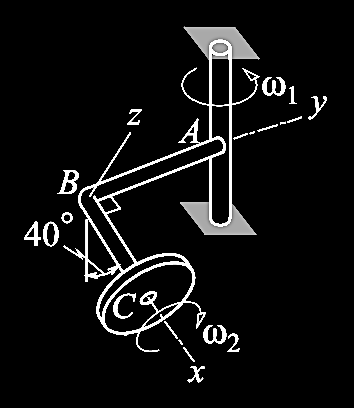
\includegraphics[frame]{images/Q3_28.png}
\end{figure}}

\subsubsection*{(a) Describe the angular velocity of the rotor in terms of a superposition of simple rotations.}

Sketching out the frames of rotation relative to each other:

\begin{center}
\tikzset{
pattern size/.store in=\mcSize, 
pattern size = 5pt,
pattern thickness/.store in=\mcThickness, 
pattern thickness = 0.3pt,
pattern radius/.store in=\mcRadius, 
pattern radius = 1pt}
\makeatletter
\pgfutil@ifundefined{pgf@pattern@name@_3f955ijae}{
\pgfdeclarepatternformonly[\mcThickness,\mcSize]{_3f955ijae}
{\pgfqpoint{-\mcThickness}{-\mcThickness}}
{\pgfpoint{\mcSize}{\mcSize}}
{\pgfpoint{\mcSize}{\mcSize}}
{
\pgfsetcolor{\tikz@pattern@color}
\pgfsetlinewidth{\mcThickness}
\pgfpathmoveto{\pgfpointorigin}
\pgfpathlineto{\pgfpoint{0}{\mcSize}}
\pgfusepath{stroke}
}}
\makeatother

% Pattern Info
 
\tikzset{
pattern size/.store in=\mcSize, 
pattern size = 5pt,
pattern thickness/.store in=\mcThickness, 
pattern thickness = 0.3pt,
pattern radius/.store in=\mcRadius, 
pattern radius = 1pt}
\makeatletter
\pgfutil@ifundefined{pgf@pattern@name@_6pdewzxwt}{
\pgfdeclarepatternformonly[\mcThickness,\mcSize]{_6pdewzxwt}
{\pgfqpoint{-\mcThickness}{-\mcThickness}}
{\pgfpoint{\mcSize}{\mcSize}}
{\pgfpoint{\mcSize}{\mcSize}}
{
\pgfsetcolor{\tikz@pattern@color}
\pgfsetlinewidth{\mcThickness}
\pgfpathmoveto{\pgfpointorigin}
\pgfpathlineto{\pgfpoint{0}{\mcSize}}
\pgfusepath{stroke}
}}
\makeatother
\tikzset{every picture/.style={line width=0.75pt}} %set default line width to 0.75pt        

\begin{tikzpicture}[x=0.75pt,y=0.75pt,yscale=-1,xscale=1]
%uncomment if require: \path (0,269); %set diagram left start at 0, and has height of 269

%Straight Lines [id:da20435224588937562] 
\draw [line width=1.5]    (314,151) -- (315,61) ;
%Straight Lines [id:da03445781531687486] 
\draw    (314,151) -- (411,152) ;
%Straight Lines [id:da7893099740949647] 
\draw [line width=0.75]    (358,85) -- (314,151) ;
%Straight Lines [id:da8958798831337074] 
\draw [line width=0.75]    (314,151) -- (366,225) ;
%Straight Lines [id:da3609400739420203] 
\draw [pattern=_3f955ijae,pattern size=6pt,pattern thickness=0.75pt,pattern radius=0pt, pattern color={rgb, 255:red, 0; green, 0; blue, 0}][line width=0.75]  [dash pattern={on 4.5pt off 4.5pt}]  (314,151) -- (315,241) ;
%Curve Lines [id:da8730659221398798] 
\draw    (336,118) .. controls (334,101) and (318,103) .. (314.5,106) ;
%Curve Lines [id:da41577213022532145] 
\draw    (314.5,196) .. controls (324.5,204) and (341,186) .. (336,182) ;
%Straight Lines [id:da6094981848974355] 
\draw [pattern=_6pdewzxwt,pattern size=6pt,pattern thickness=0.75pt,pattern radius=0pt, pattern color={rgb, 255:red, 0; green, 0; blue, 0}][line width=0.75]  [dash pattern={on 4.5pt off 4.5pt}]  (314,151) -- (276,87) ;
%Curve Lines [id:da6552705712368743] 
\draw    (314.5,106) .. controls (300,101.5) and (295.5,110) .. (292,113) ;

% Text Node
\draw (366,220) node [anchor=north west][inner sep=0.75pt]   [align=left] {$x$};
% Text Node
\draw (414.54,143.31) node [anchor=north west][inner sep=0.75pt]   [align=left] {$y$};
% Text Node
\draw (360,68) node [anchor=north west][inner sep=0.75pt]   [align=left] {$z$};
% Text Node
\draw (308,43) node [anchor=north west][inner sep=0.75pt]   [align=left] {$Z$};
% Text Node
\draw (298,144) node [anchor=north west][inner sep=0.75pt]   [align=left] {$C$};
% Text Node
\draw (313.5,177) node [anchor=north west][inner sep=0.75pt]   [align=left] {{\scriptsize $40^\circ$}};
% Text Node
\draw (315.0,109) node [anchor=north west][inner sep=0.75pt]   [align=left] {{\scriptsize $50^\circ$}};
% Text Node
\draw (295.5,107) node [anchor=north west][inner sep=0.75pt]   [align=left] {{\scriptsize $40^\circ$}};

\end{tikzpicture}
\end{center}

Constructing the angular velocity vector $\bar{\omega}$ of $xyz$ by vectorially adding the simple rotation rates according to:

$$ \bar{\omega} = \omega_1 \bar{e}_1 + \omega_2 \bar{e}_2$$

This gives us:

$$ \bar{\omega} = \omega_1 \bar{K} + \omega_2 (-\bar{i})$$

Or:

\begin{answer}
$$ \bar{\omega} = \omega_1 \bar{K} +  \omega_2 \bar{i}$$
\end{answer}

\subsubsection*{(b) Solely from an examination of the description in Part (a), predict the direction(s) in which the angular acceleration of the rotor will be situated relative to the xyz axes defined in the sketch. Briefly explain your answer.}

In terms of the reference frame $xyz$, the angular acceleration is only affected by the constant rotations of $\omega_1$ and $\omega_2$.
% Therefore, the only angular acceleration experienced by the rotor is due to change in orientation relative to the reference frame.
The angular acceleration component of $\omega_2$ is in the negative in the ${i}$ direction.
The component of the rotation $\omega_1$ that is perpendicular to the rotor axis is $\omega_1 \cos(50)$.
The vector cross of these two vectors results in an acceleration of in the $-j$ direction.
All together the acceleration is:

\begin{answer}
    $$ \bar{\alpha} = \omega_1 \omega_2 \cos(50^\circ) \left(-\bar{j}\right) $$
\end{answer}

\subsubsection*{(c) Describe the angular velocity and angular acceleration of the rotor in terms of components relative to xyz.}

Because the first auxiliary reference frame is stationary, and the second one is $xyz$, we have:

$$ \bar{\Omega}_1 = \bar{0}, \ \ \bar{\Omega}_2 = \bar{\omega} $$

We find the global components of the unit vectors by inspection of the sketch, which leads to

\begin{equation*}
\begin{aligned}
\bar{K} &= \cos(40^\circ)(-\bar{i}) + \cos(50^\circ)\bar{k} \\
        &= -\cos(40^\circ)\bar{i} + \cos(50^\circ)\bar{k}  \\
\bar{i} &= \bar{i} 
\end{aligned}
\end{equation*}

This makes the velocity:

\begin{answer}
$$ \bar{\omega} = \left(\omega_2-\cos(40^\circ)\omega_1\right) \bar{i} + \omega_1\cos(50^\circ)\bar{k} $$
\end{answer}

Next solve for angular acceleration:

$$ \bar{\alpha} =
\sum_n \left( \dot{\omega}_n \bar{e}_n + \bar{\Omega}_n \times \omega_n \bar{e}_n \right) $$

Since $n=2$:

$$ \bar{\alpha} =
\dot{\omega}_1 \bar{e}_1 + \bar{\Omega}_1 \times \omega_1 \bar{e}_1 +
\dot{\omega}_2 \bar{e}_2 + \bar{\Omega}_2 \times \omega_2 \bar{e}_2 $$

And since $\dot{\omega}_1 = \dot{\omega}_2 = 0$:

$$ \bar{\alpha} =
\bar{\Omega}_1 \times \omega_1 \bar{e}_1 +
\bar{\Omega}_2 \times \omega_2 \bar{e}_2 $$

Futher, as stated above that $\bar{\Omega}_1 = \bar{0}$ and $\bar{\Omega}_2 = \bar{\omega}$:

\begin{equation*}
\begin{aligned}
\bar{\alpha} &= \bar{\Omega}_2 \times \omega_2 \bar{e}_2\\
             &= \left( \left(\omega_2-\cos(40^\circ)\omega_1\right) \bar{i} + \omega_1\cos(50^\circ)\bar{k} \right)
                \times \omega_2 (-\bar{i})\\
            &= -\omega_2 \left( \left(\omega_2-\cos(40^\circ)\omega_1\right) \bar{i} + \omega_1\cos(50^\circ)\bar{k} \right)
                \times \bar{i}\\
\end{aligned}
\end{equation*}

Which solves to:

\begin{answer}
$$ \bar{\alpha} = -\omega_1 \omega_2 \cos(50^\circ) \bar{j} $$
\end{answer}

\subsection*{EXERCISE 3.37}
\subsubsection*{The angle $\bm{\theta}$ describing the rotation of a reconnaissance satellite's solar panels about the body-fixed $\bm{x}$ axis is an arbitrary function of time.
The satellite spins about the $\bm{z}$ axis at the constant rate $\bm{\Omega}$.
Derive expressions for the absolute velocity and acceleration of point $\bm{B}$ relative to the origin of $\bm{xyz}$.
\begin{figure}[H]
    \centering
    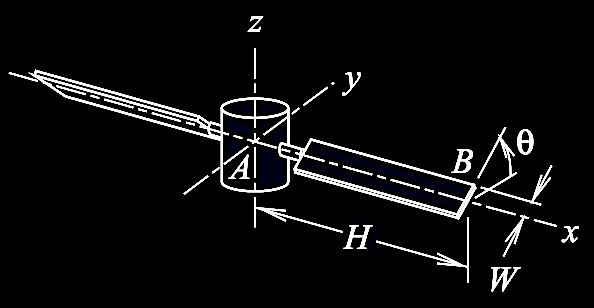
\includegraphics[frame]{images/Q3_37.png}
\end{figure}}

This problem can be defined in terms of three reference frames: the inertially fixed $\{XYZ\}$ frame, the satellite body fixed frame $\{xyz\}$, and a frame defining the rotation of the solar panel relative to the satellite body frame $\{x'y'z'\}$.
These are all detailed in the following diagram:


\begin{center}
\tikzset{every picture/.style={line width=0.75pt}} %set default line width to 0.75pt        

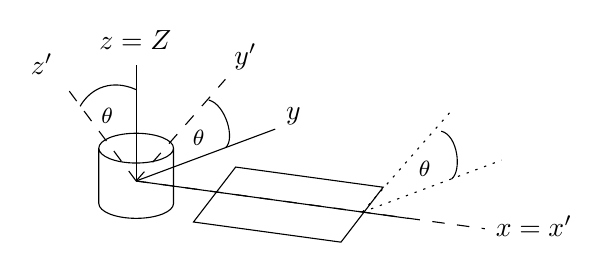
\begin{tikzpicture}[x=0.75pt,y=0.75pt,yscale=-1,xscale=1]

%Flowchart: Magnetic Disk [id:dp3635321013642623] 
\draw   (219,105.18) -- (219,131.82) .. controls (219,135.79) and (210.94,139) .. (201,139) .. controls (191.06,139) and (183,135.79) .. (183,131.82) -- (183,105.18)(219,105.18) .. controls (219,109.14) and (210.94,112.35) .. (201,112.35) .. controls (191.06,112.35) and (183,109.14) .. (183,105.18) .. controls (183,101.21) and (191.06,98) .. (201,98) .. controls (210.94,98) and (219,101.21) .. (219,105.18) -- cycle ;
%Flowchart: Data [id:dp3120937293163366] 
\draw   (248.94,114.29) -- (320,124) -- (299.68,150.47) -- (228.62,140.76) -- cycle ;
%Straight Lines [id:da5131444866807715] 
\draw    (201,121) -- (332,139) ;
%Straight Lines [id:da3197855635030902] 
\draw  [dash pattern={on 4.5pt off 4.5pt}]  (201,121) -- (369,144) ;
%Straight Lines [id:da9045678164619011] 
\draw    (201,121) -- (201,65) ;
%Straight Lines [id:da1980514691616675] 
\draw    (201,121) -- (268,96) ;
%Straight Lines [id:da15286153807833958] 
\draw  [dash pattern={on 4.5pt off 4.5pt}]  (201,121) -- (244,72) ;
%Curve Lines [id:da34869742372984613] 
\draw    (236,82) .. controls (244,84) and (249,101) .. (244,105) ;
%Straight Lines [id:da2648942609548608] 
\draw  [dash pattern={on 0.84pt off 2.51pt}]  (310,136) -- (377,111) ;
%Straight Lines [id:da8634219746067795] 
\draw  [dash pattern={on 0.84pt off 2.51pt}]  (310,136) -- (353,87) ;
%Curve Lines [id:da1290081440816302] 
\draw    (348,97) .. controls (356,99) and (358,116) .. (353,120) ;
%Straight Lines [id:da32191607843243353] 
\draw  [dash pattern={on 4.5pt off 4.5pt}]  (201,121) -- (166,74) ;
%Curve Lines [id:da41691895480714614] 
\draw    (174,85) .. controls (179.5,75.5) and (190,72) .. (201,77) ;

% Text Node
\draw (373,136.4) node [anchor=north west][inner sep=0.75pt]    {$x=x'$};
% Text Node
\draw (182,47.4) node [anchor=north west][inner sep=0.75pt]    {$z=Z$};
% Text Node
\draw (227,95.4) node [anchor=north west][inner sep=0.75pt]  [font=\footnotesize]  {$\theta $};
% Text Node
\draw (272,84.4) node [anchor=north west][inner sep=0.75pt]    {$y$};
% Text Node
\draw (247,53.4) node [anchor=north west][inner sep=0.75pt]    {$y'$};
% Text Node
\draw (336,110.4) node [anchor=north west][inner sep=0.75pt]  [font=\footnotesize]  {$\theta $};
% Text Node
\draw (183,84.4) node [anchor=north west][inner sep=0.75pt]  [font=\footnotesize]  {$\theta $};
% Text Node
\draw (149,58.4) node [anchor=north west][inner sep=0.75pt]    {$z'$};

\end{tikzpicture}

\end{center}


Construct the angular velocity vector $\bar{\omega}$ of $xyz$ by vectorially adding the simple rotation rates according to:

$$ \bar{\omega} = \omega_1 \bar{e}_1 + \omega_2 \bar{e}_2$$

This gives us:

$$ \bar{\omega} = \Omega\ \bar{K} + \dot{\theta}\ \bar{i}'$$

We find the global components of the unit vectors by inspection of the sketch, which leads to

\begin{equation*}
\begin{aligned}
    \bar{i}' &=\bar{i} \\
    \bar{K} &= \bar{k}
\end{aligned}
\end{equation*}

This gives us:

$$ \bar{\omega} = \dot{\theta}\ \bar{i}  +\Omega \bar{k} $$

Next solve for angular acceleration:

$$ \bar{\alpha} =
\sum_n \left( \dot{\omega}_n \bar{e}_n + \bar{\Omega}_n \times \omega_n \bar{e}_n \right) $$

Since $n=2$:

$$ \bar{\alpha} =
\dot{\omega}_1 \bar{e}_1 + \bar{\Omega}_1 \times \omega_1 \bar{e}_1 +
\dot{\omega}_2 \bar{e}_2 + \bar{\Omega}_2 \times \omega_2 \bar{e}_2 $$

And since $\dot{\omega}_1 = 0$:

$$ \bar{\alpha} =
\bar{\Omega}_1 \times \omega_1 \bar{e}_1 +
\dot{\omega}_2 \bar{e}_2 + \bar{\Omega}_2 \times \omega_2 \bar{e}_2 $$

Because the there is only a $z$ rotation for the frame $xyz$,
and the frame $x'y'z'$ experience the full system rotation:

$$ \bar{\Omega}_1 = \Omega, \ \ \bar{\Omega}_2 = \bar{\omega} $$

Therefore,

\begin{equation*}
\begin{aligned}
\bar{\alpha} &= \cancelto{0}{\Omega \bar{k} \times \Omega \bar{k}} + \dot{\theta} \bar{i}  + \bar{\omega} \times \dot{\theta} \bar{i} \\
             &= \ddot{\theta}\bar{i} + \Omega \,\dot{\theta} \bar{j}
\end{aligned}
\end{equation*}

The relative position to B from A is computed as:

$$ \bar{r}_{B/A} = \left[\begin{array}{r} H \ \bar{i}\\
    W\,\cos\left(\theta\right) \ \bar{j}\\
    W\,\sin\left(\theta\right) \ \bar{k}
\end{array}\right] $$

Given this, we can solve for the absolute velocity of B relative to the origin as:

\begin{equation*}
    \begin{aligned}
    \bar{v}_B &= \cancelto{0}{\bar{v}_A} + \bar{\omega} \times \bar{r}_{B/A} \\
                 &= \left[\begin{array}{r} -\Omega \,W\,\cos\left(\theta\right) \bar{i}\\
                    H\,\Omega -W\,\sin\left(\theta\right)\,\dot{\theta} \bar{j}\\
                    W\,\cos\left(\theta\right)\,\dot{\theta} \bar{k}
                \end{array}\right]
    \end{aligned}
\end{equation*}

So,

\begin{answer}
    \begin{equation*}
        \begin{aligned}
        \bar{v}_B &= \left[\begin{array}{r} -\Omega \,W\,\cos\left(\theta\right) \bar{i}\\
            H\,\Omega -W\,\sin\left(\theta\right)\,\dot{\theta} \bar{j}\\
            W\,\cos\left(\theta\right)\,\dot{\theta} \bar{k}
        \end{array}\right]
        \end{aligned}
    \end{equation*}
\end{answer}

We can also compute the absolute acceleration of B relative to the origin as:

\begin{equation*}
    \begin{aligned}
    \bar{a}_B &= \cancelto{0}{\bar{a}_A} + \bar{\alpha} \times \bar{r}_{B/A} + \bar{\omega} \times \left( \bar{\omega} \times \bar{r}_{B/A} \right)  \\
              &= \left[\begin{array}{r} \left\{ 2\,\Omega \,\dot{\theta}\,\sin\left(\theta\right)\,W-H\,\Omega ^2 \right\} \bar{i} \\
                       \left\{ -\left({\dot{\theta}}^2+\Omega ^2\right)\,\cos\left(\theta\right)\,W-\ddot{\theta}\,\sin\left(\theta\right)\,W \right\} \bar{j} \\
                       \left\{ \ddot{\theta}\,\cos\left(\theta\right)\,W-{\dot{\theta}}^2\,\sin\left(\theta\right)\,W \right\} \bar{k}
                    \end{array}\right]
    \end{aligned}
\end{equation*}

So,

\begin{answer}
    \begin{equation*}
        \begin{aligned}
        \bar{a}_B = \left[\begin{array}{r} \left\{ 2\,\Omega \,\dot{\theta}\,\sin\left(\theta\right)\,W-H\,\Omega ^2 \right\} \bar{i} \\
                           \left\{ -\left({\dot{\theta}}^2+\Omega ^2\right)\,\cos\left(\theta\right)\,W-\ddot{\theta}\,\sin\left(\theta\right)\,W \right\} \bar{j} \\
                           \left\{ \ddot{\theta}\,\cos\left(\theta\right)\,W-{\dot{\theta}}^2\,\sin\left(\theta\right)\,W \right\} \bar{k}
                        \end{array}\right]
        \end{aligned}
    \end{equation*}
\end{answer}

% \color{white}
% \hspace*{6em}\inputminted[frame=leftline,fontsize=\footnotesize]{matlab}
% {./matlab/B_2_18.m}
% \color{black} 

% It has the following response, which matches my analytically derived solution:

% \begin{figure}[H]
%     \centering
%     \includegraphics{matlab/B_2_18.png}
%     \caption{Response of the system}
% \end{figure}

\end{document}

